
\documentclass[11pt,a4paper]{article}
\usepackage[utf8]{inputenc}
%\usepackage[icelandic]{babel}
%\usepackage[T1]{fontenc}
\usepackage{amsmath}
\usepackage{amsfonts}
\usepackage{amssymb}
%\usepackage{graphicx}
%\author{Arnar Ingi Halldórsson}
%\title{Linear Motion}


%\documentclass{article}
\usepackage{graphicx}
\graphicspath{ {myndir/} }
\usepackage[T1]{fontenc} 
\usepackage[english]{babel}

\usepackage[utf8]{inputenc} 
\usepackage{graphics}
%\usepackage[pdftex]{graphicx}

\usepackage{caption}
\usepackage{subcaption}
\usepackage[top=2in, bottom=1.5in, left=1in, right=1in]{geometry}
%\usepackage{titling}

%\setlength{\droptitle}{-10em}
   
\title{Assignment 1 \\ T-509-RAFT \\ Electronics} % Title

\author{Arnar Ingi Halldórsson \\ Hjörleifur G. Bergsteinsson \\ Snorri Stefánsson} % Author name
\begin{document}

\maketitle % Insert the title, author and date

\begin{tabular}{lr}
Due date: 22.02.2015 \\
Teachers:\qquad Slawomir Koziel\\ % Instructor/supervisor
\qquad \qquad \qquad Adrian Bekasiewicz
\end{tabular}

\setlength\parindent{0pt} % Removes all indentation from paragraphs

\renewcommand{\labelenumi}{\alph{enumi}.} % Make numbering in the enumerate environment by letter rather than number (e.g. section 6)

\section*{Introduction}


\section*{Task 1: Perfomance Parameters of Op Amp}

\begin{enumerate}
  \item[1.]
  The circuit diagram shown below was simulated in $MultiSim$ to find the slew-rate(SR) of a op amp.\\
    \begin{minipage}{\linewidth}
      \centering       
       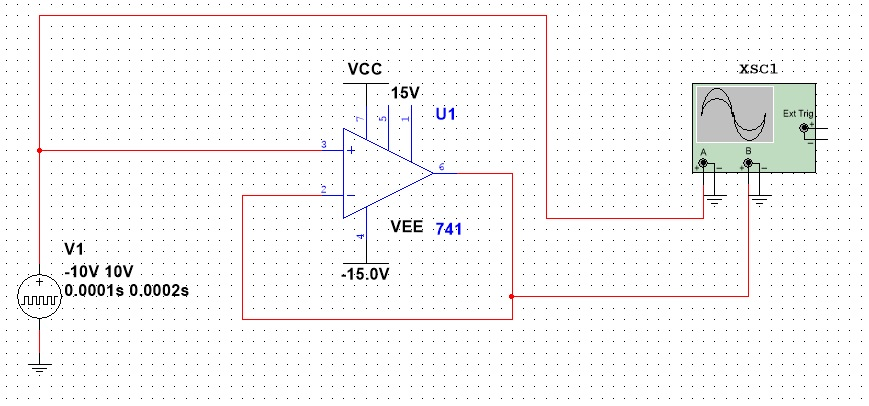
\includegraphics[width=10cm]{Task1-1Circuit}\\
     \captionof{figure}{yoyo} 
    \end{minipage}\\
\pagebreak
\pagebreak

In Fig 2 shows the measurements from the Oscilloscope. The diagram shows the effect of the slew rate limiting on the output rectangular waveform.\\
    \begin{minipage}{\linewidth}
      \centering       
       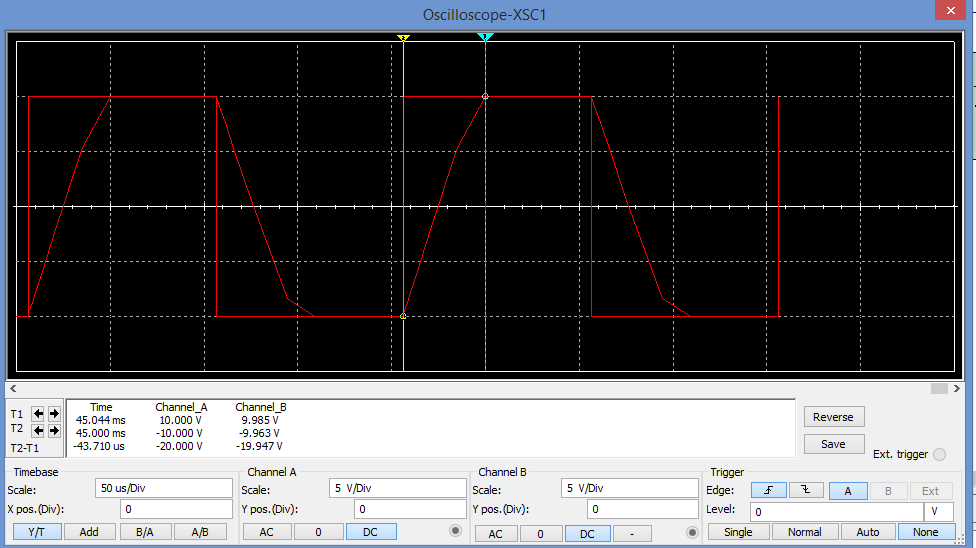
\includegraphics[width=10cm]{Task1-1-Oscilloscope}\\
      \captionof{figure}{} 
    \end{minipage}
$$ \dfrac{dv_{o}}{dt}|_{max} = \dfrac{-19.947 \ V}{-43.719\ \mu s} = 0.456 \frac{V}{\mu s} $$
  \item[2.]
  The circuit diagram shown below was simulated with AC analysis to determine the gain-bandwidth product(GBW) of the op amp.  
  
      \begin{minipage}{\linewidth}
      \centering
        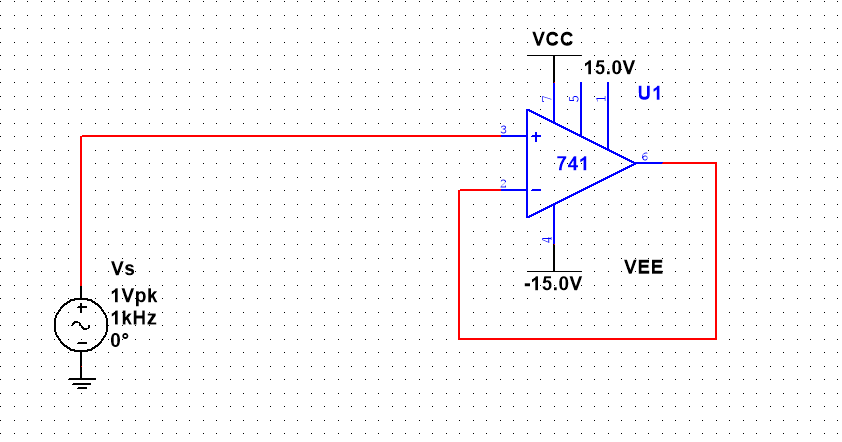
\includegraphics[width=10cm]{Task1-2-Circuit}\\
    \captionof{figure}{} 
    \end{minipage}
    
   In Fig 4 shows the measurements from the AC analysis of the circuit. 
    $$ BW \simeq f_{H} $$
    $$ GB = |A_{G}|BW $$
    
    The gain is unity gain buffer because of the voltage follower. 
    $$ GB = BW $$
    
    The $f_{H}$ is 995.486 kHz in Fig 4. So the gain-bandwidth product is
    $$ GB = 995.486  kHz$$
    
    \begin{minipage}{\linewidth}
      \centering
        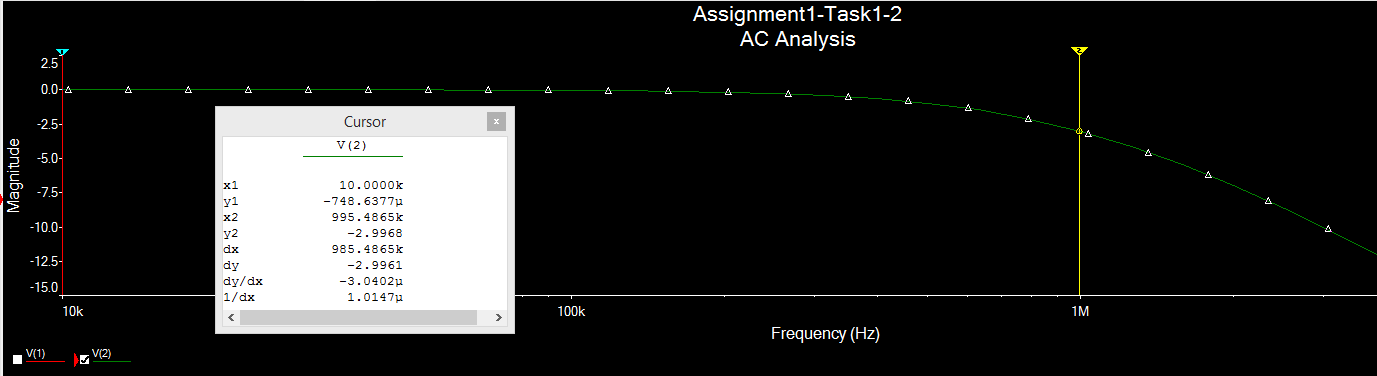
\includegraphics[width=14cm]{Task1-2-ACAnalysis}\\
    \captionof{figure}{}     
    \end{minipage}
  %     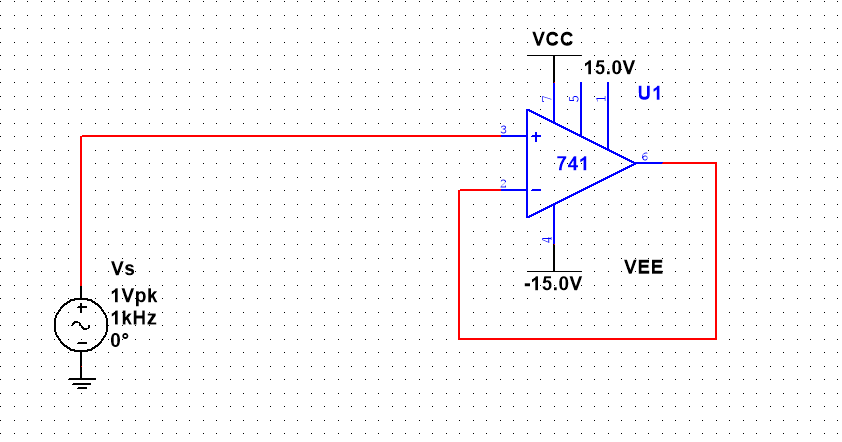
\includegraphics[width=10cm]{Task1-2-Circuit}\\
    % 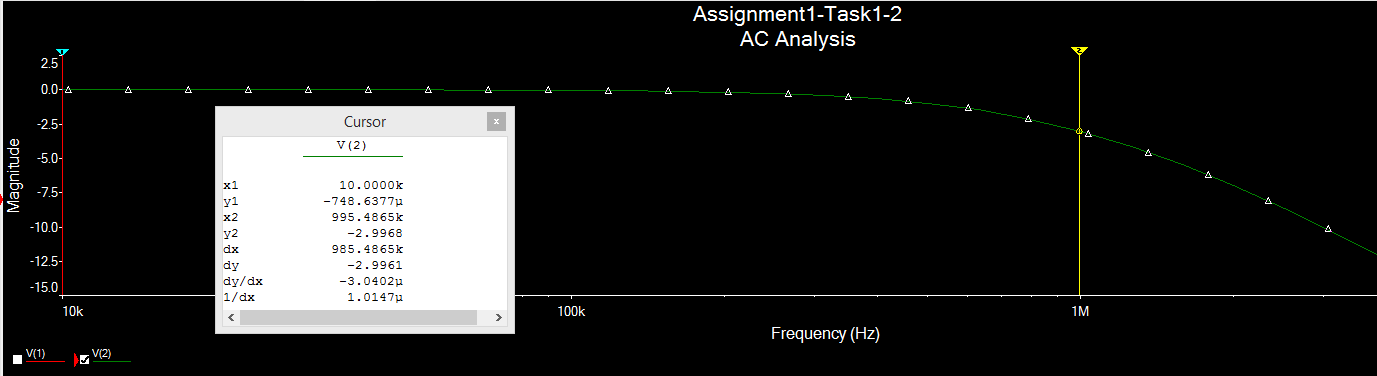
\includegraphics[width=10cm]{Task1-2-ACAnalysis}\\
  \item[3.]
  
  
  The circuit below was simulated in MultiSim to determine the DC differential gain $A_{d}$ and the input offset voltage $V_{OS}$ of the op amp.
  
      \begin{minipage}{\linewidth}
      \centering
      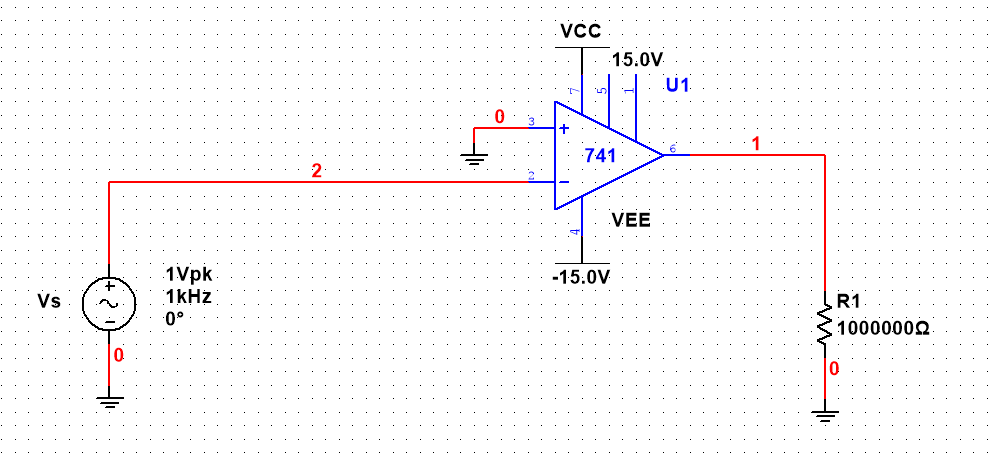
\includegraphics[width=10cm]{Task1-3-Circuit}\\
    \captionof{figure}{}   
    \end{minipage}
    
In Fig 6 show the result of the DC analysis of the circuit in Fig 5. Hence that the DC differential gain is
$$A_{d} = 206.505 \frac{V}{mV} $$    
    
    
        \begin{minipage}{\linewidth}
      \centering
      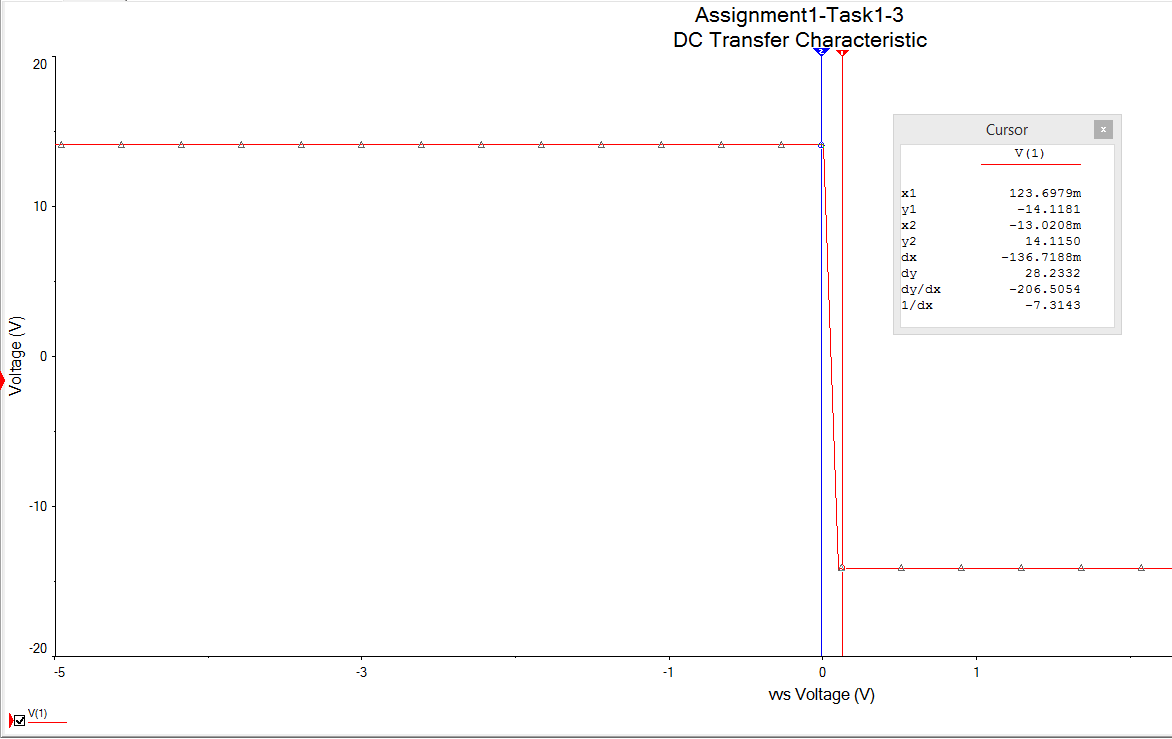
\includegraphics[width=10cm]{Task1-3-DCAnalysis}\\
    \captionof{figure}{}    
    \end{minipage}\\   
In Fig 7 shows the result of the DC analysis and hence the offset Voltage can be determine to be
$$ V_{OS} = 1.147 mV $$\\
    
    
\begin{minipage}{\linewidth}
  \centering
    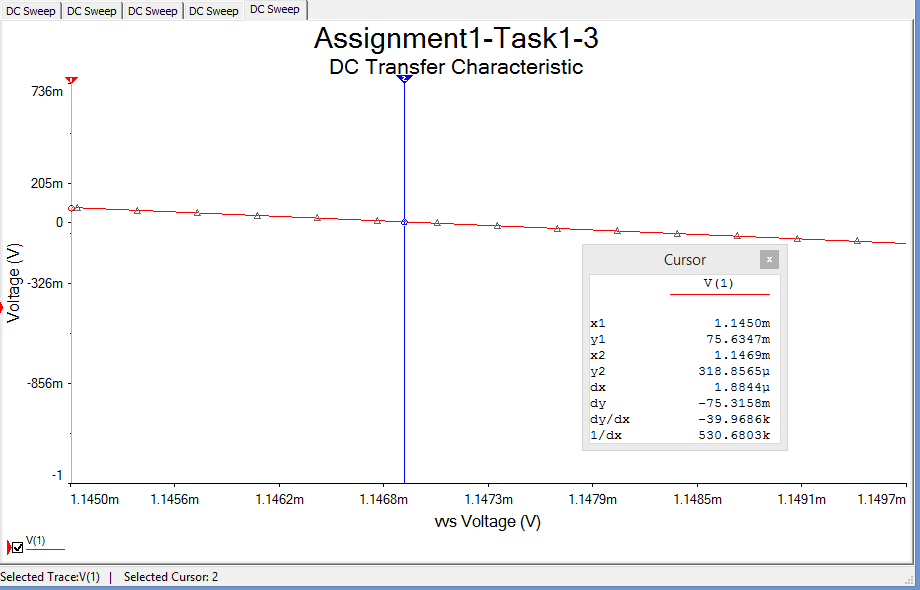
\includegraphics[width=10cm]{Task1-3-Vos}\\
    \captionof{figure}{}    
    \end{minipage}\\
    
    
 \item[4.]
 

Diffrence between theoretical values and simulated values of the $\mu A741$ op amp can be seen in table 1.\\

\begin{minipage}{\linewidth}

\begin{center}
  \begin{tabular}{r l r l r l}
	\multicolumn{2}{c}{$\mu$A741 op-Amp} &   
  \multicolumn{2}{c}{DataSheet} &
  \multicolumn{2}{c}{Simulation}\\
  \hline
    Slew Rate & [$SR$] & 0.5 & $ [\frac{V}{\mu s}]$ & 0.456& $      [\frac{V}{\mu s}]$ \\
  Gain-Bandwidth & [$GBW$]& 1 &$ [MHz]$  & 995.487 &$ [MHz]$ \\
  DC Differential Gain &[$A_{d}$] & 200& $[\frac{V}{mV}]$ & 206.505& $[\frac{V}{mV}]$ \\
  Input Offset Voltage &[$V_{os}$] & 5& $[mV]$& 1.147& $[mV]$ \\
    \end{tabular}
    \captionof{table}{Theoretical and simulated values of $\mu$A741 op amp}
\end{center}
\end{minipage}
\end{enumerate}

\section*{Task 2: Frequency Response of Inverting Amplifier}

\begin{enumerate}
  \item[1.]
  
  Figure below shows the inverting amplifier that we simulated in MultiSim. The task was to determine the 3dB corner frequency of the op amp with AC analysis.\\
  \begin{minipage}{\linewidth}
  \centering
      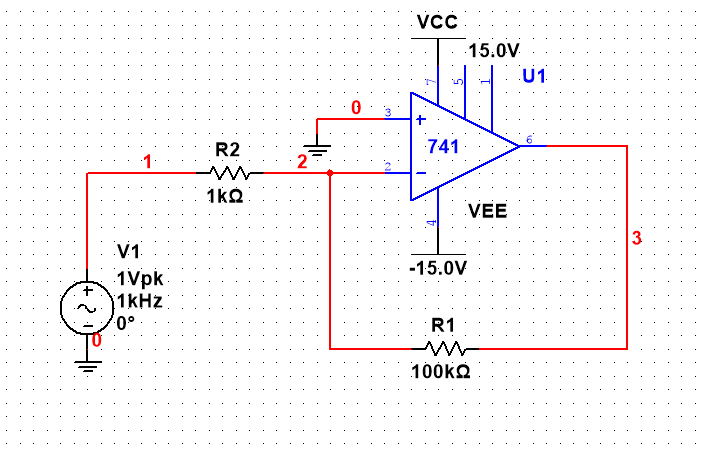
\includegraphics[width=10cm]{Task2-1-Circuit}\\
    \captionof{figure}{}    
    \end{minipage}\\
Figure 9 shows the AC analysis and hence the 3dB  frequency is
$$ f_{3dB} = 9.910 \ kHz $$
  \begin{minipage}{\linewidth}
  \centering
      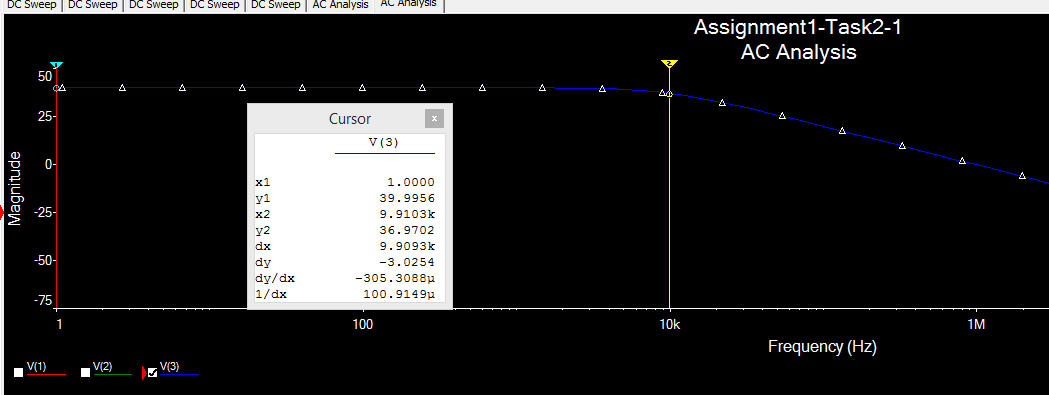
\includegraphics[width=14cm]{Task2-1-ACAnalysis}\\
    \captionof{figure}{}    
    \end{minipage}\\

  \item[2.]
  By using the theoretical values to compare to simulated result of the 3 dB frequency.
$$f_{t} = A_{t}w_{b}$$
$$ f_{b} = \frac{f_{t}}{A_{b}} = \frac{1\ MHz}{100 \frac{V}{V}} = 10\ kHz $$
Which is close to the simulated value from the AC analysis.  

\end{enumerate}
\pagebreak
\section*{Task 3: Op Amplifies Design}

\begin{enumerate}
  \item[1.]
  An op-amp-based integrator was designed with the dc gain equal to -10 V/V where \\R1 = 200$\Omega$ and R2 = 2k$\Omega$ as can be seen in fig X. The value of the capacitance C of the integrator was calculated so that its 3dB frequency is 50kHz. %Knowing the gain bandwith product of the $\mu$A741 op amp to be 1MHz the capacitance can be calculated with the following formula.
$$\omega_0 = \frac{1}{C\cdot R_2} \Leftrightarrow C = \frac{1}{\omega_0 \cdot R_2} \Leftrightarrow C  = \frac{1}{50\text{kHz}\cdot 2\pi \cdot 2k\Omega} = 1.592 nF $$
  \begin{minipage}{\linewidth}
    	\centering       
        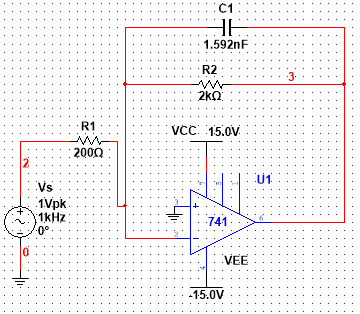
\includegraphics[width=7cm]{Task3_1.png}
        \captionof{figure}{Circuit diagram of an op-amp-based integrator} 
    \end{minipage}
  \item[2.]
  Simulation of the integrator seen in fig X, shows that the 3dB frequency is 33.8kHz. This is not as predicted by theory from task 3.1. Previous calculations were done assuming an ideal amplifier which is not correct. There is a significant difference between the result and the expected result so further analysis must me done to find the correct value of the capacitance C so that the 3dB frequency will be 50kHz.\\
  \begin{minipage}{\linewidth}
    	\centering       
        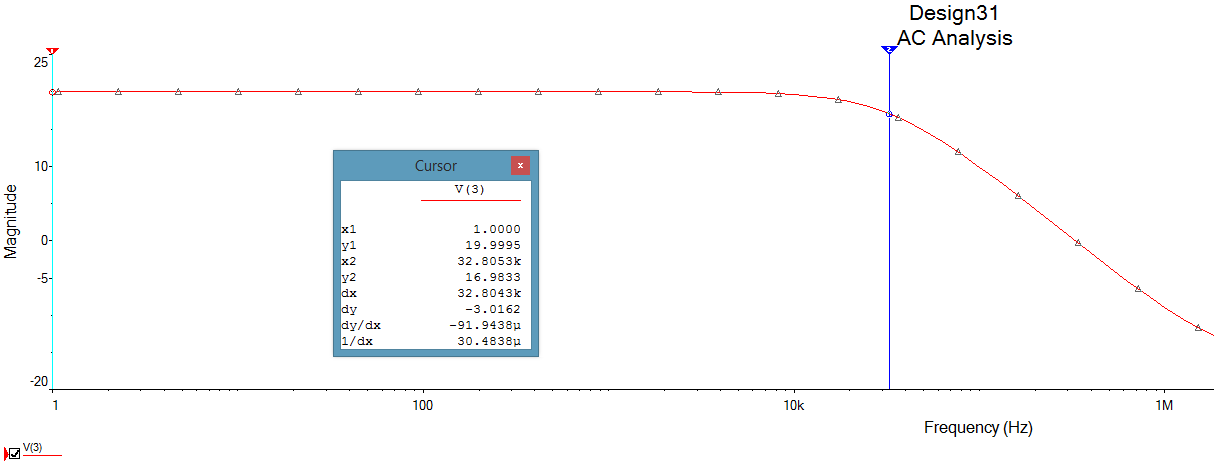
\includegraphics[width=14cm]{Task3_2.png}
        \captionof{figure}{AC analysis of the op-amp-based integrator with C = 1.592nF. } 
    \end{minipage} 
    \pagebreak
  \item[3.]
  The capacitance was determined again neglecting the finite GBW. Assuming that the gain will reach zero dB, the transfer function is equal to one since log(1) = 0 dB. 
  $$\| \frac{V_o(j\omega)}{V_i(j\omega)} \| = \| \frac{\frac{R_2}{R_1}}{1+j\omega \cdot C \cdot R_2} \| = \frac{\frac{2k\Omega}{200\Omega}}{\sqrt{1^2+(10^6 \cdot 2\pi \cdot C \cdot 2k\Omega)^2}} = 1$$
  $$\Leftrightarrow C = \sqrt{\frac{\frac{R_2}{R_1}^2-1}{(\omega \cdot R_2)^2}}  = \sqrt{\frac{10^2-1}{(10^6 \cdot 2\pi \cdot 2k\Omega)^2}} = 0.792nF$$
  
Performing the AC analysis as in task 3.1 the 3dB frequency is found to be 48.66kHz as shown in fig X.\\
\begin{minipage}{\linewidth}
    	\centering       
        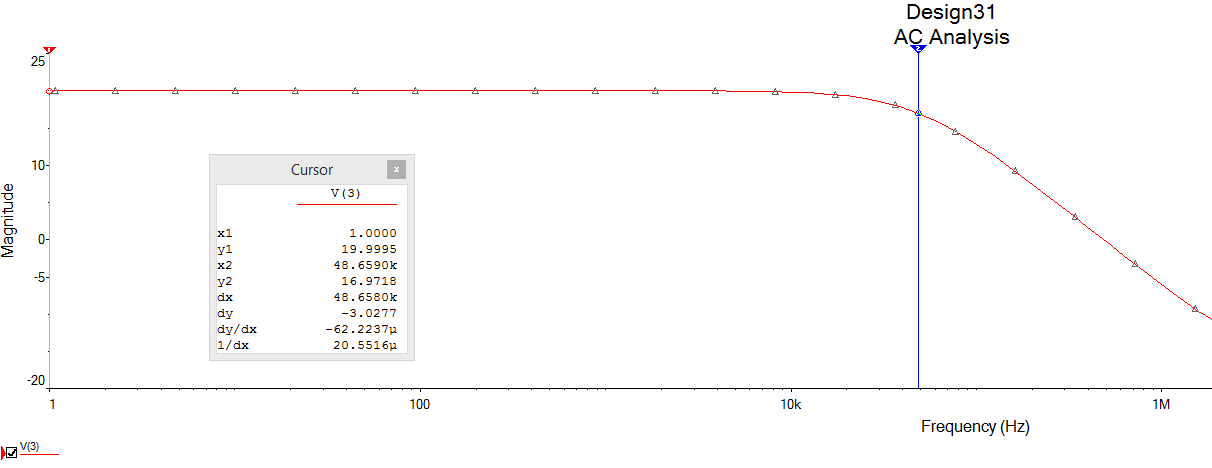
\includegraphics[width=14cm]{Task3_3.png}
        \captionof{figure}{AC analysis of the op-amp-based integrator with C = 0.792nF. } 
    \end{minipage}
\end{enumerate}
\pagebreak
\section*{Task 4: Half - Wave Rectifier}

\begin{enumerate}
  \item[$\bold{1.}$]
  Here is the half-wave rectifier circuit:
  \\
  
	\begin{minipage}{\linewidth}
    	\centering
		\captionof{figure}{}        
        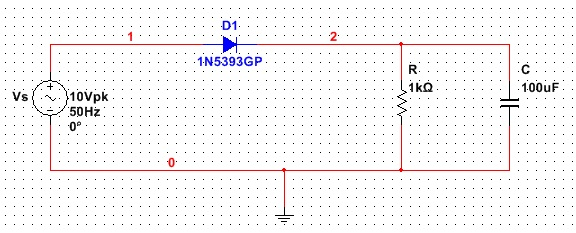
\includegraphics[width=13cm]{4_1.jpg}
    \end{minipage}
    
  
  \item[$\bold{2.}$]
  Now lets do a transient analysis of the circuit:
  \\
	\begin{minipage}{\linewidth}
    	\centering
		\captionof{figure}{Transient analysis of circuit the circuit in the last figure.}        
        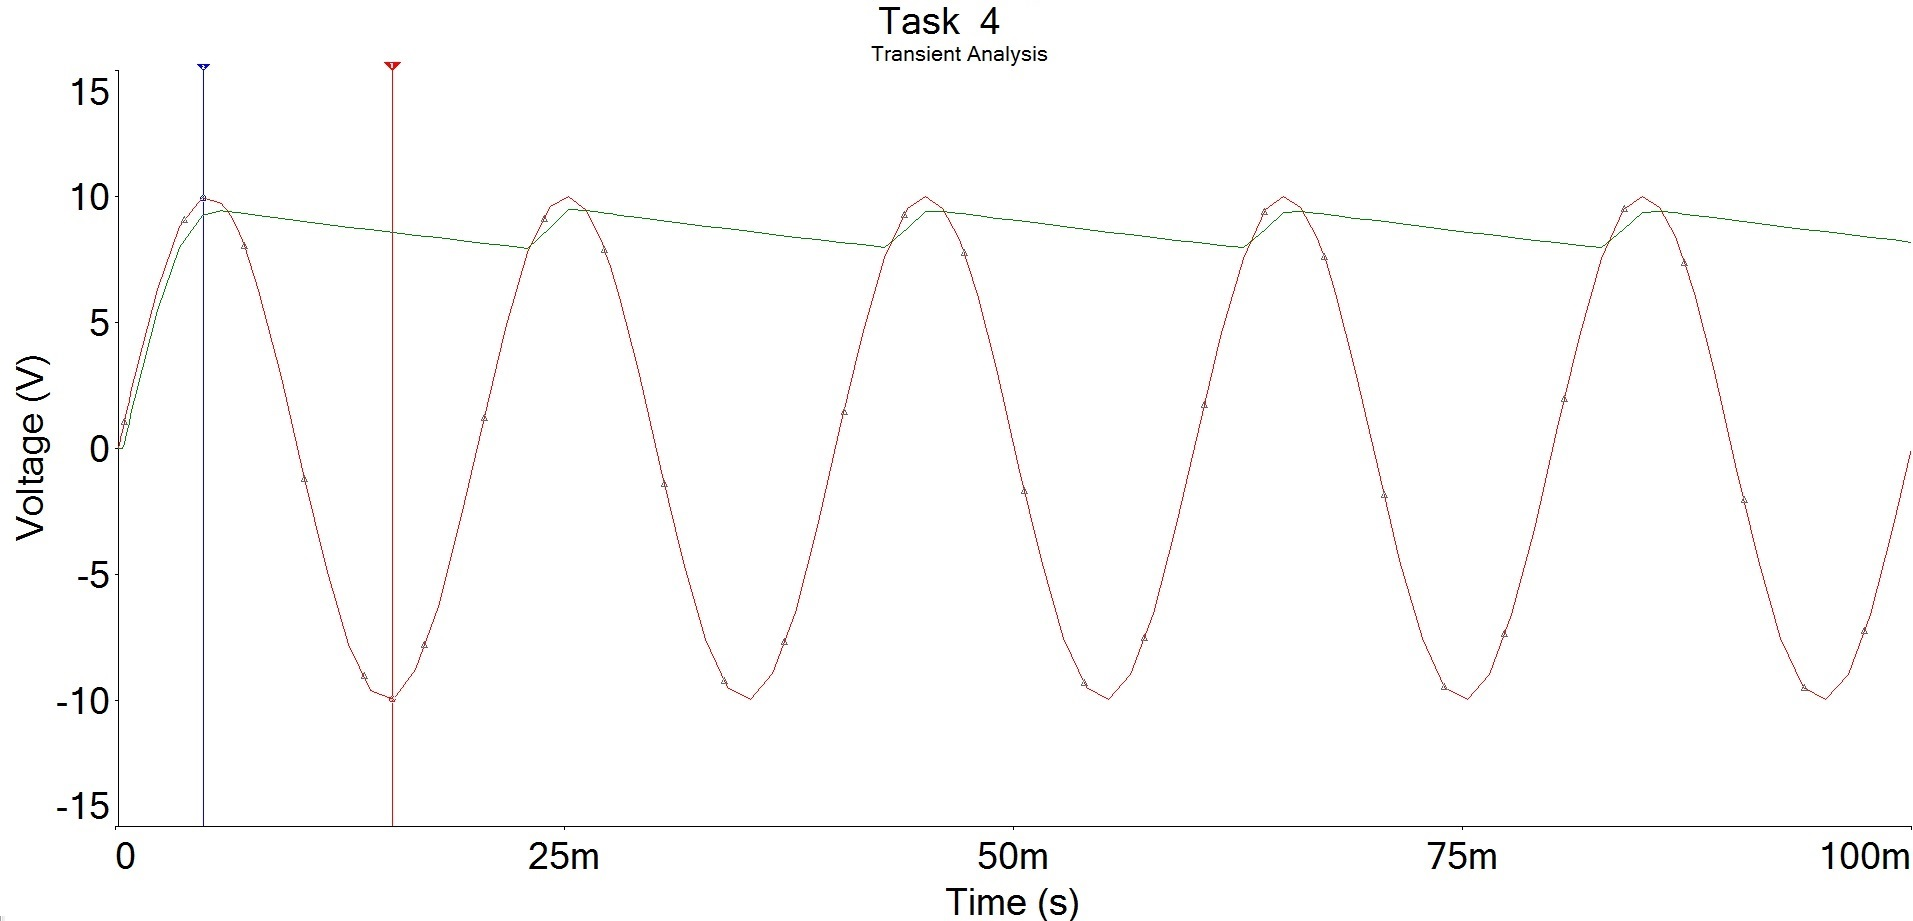
\includegraphics[width=13cm]{4_2.jpg}
    \end{minipage}

    \pagebreak
    The data for the cursors on the previous figure:\\
    
    \begin{minipage}{\linewidth}
    	\centering
		\captionof{figure}{}        
        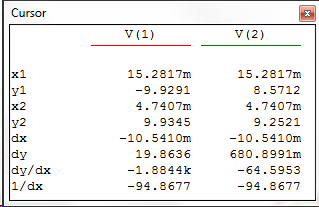
\includegraphics[width=9cm]{table_4_1.png}
    \end{minipage}
    
    \vspace{2em}
        
    So the peak voltage is y2 in the table above. That is $V_p = 9.935 V$ 
    
    The theoretical value was defined as $V_p = 10 V$ \\
    
    \begin{minipage}{\linewidth}
    	\centering
		\captionof{figure}{}        
        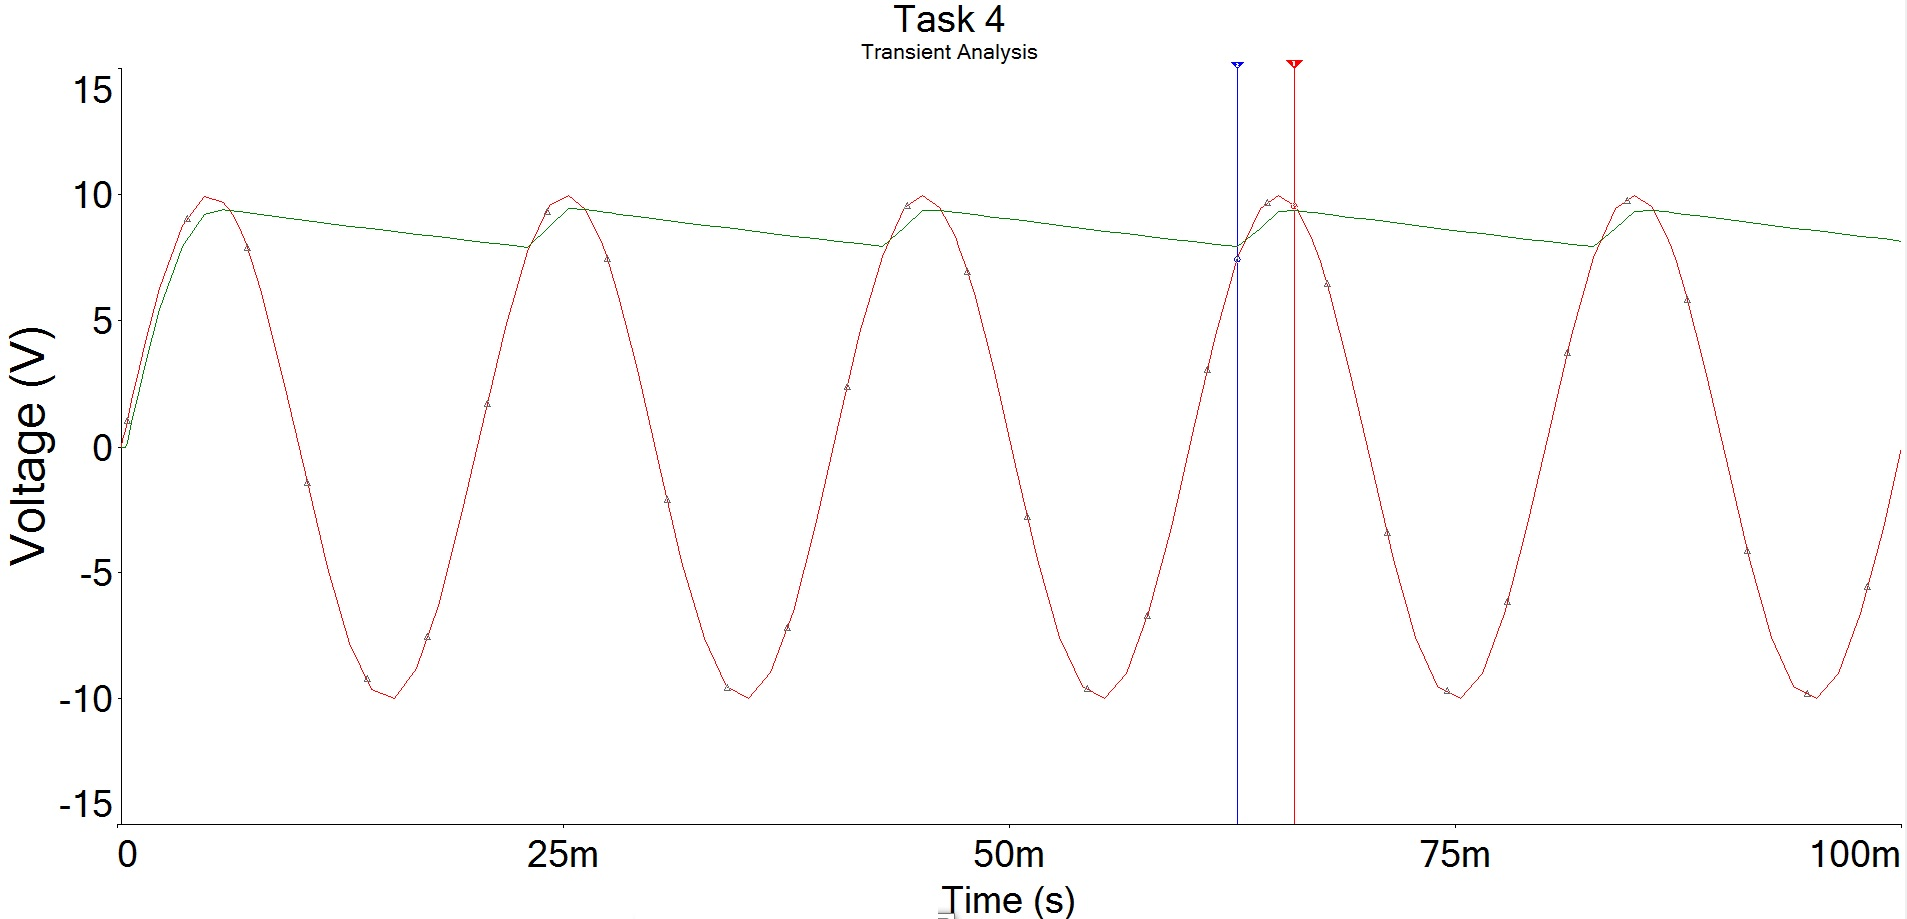
\includegraphics[width=13cm]{4_3.jpg}
    \end{minipage}
    
    \begin{minipage}{\linewidth}
    	\centering
		\captionof{figure}{}        
        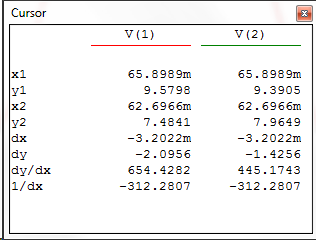
\includegraphics[width=9cm]{table_4_2.png}
    \end{minipage}
    
    \vspace{2em}
    
	The ripple voltage can be calculated from the graph. The maximum difference in voltage over the diode over one period is the ripple voltage so it can simply be seen from the graph and table, using the cursors: $$ V_r = 9.5798 V - 7.4841 V = 2.096 V$$
    The theoretical ripple voltage value can be calculated with: $$ V_r = \dfrac{V_p}{fCR} = \dfrac{10}{50 \cdot 100 \cdot 10^{-6} \cdot 10^3} = 2 V$$
    \vspace{2em}
  
  \item[$\bold{3.}$]
  
  	The ripple voltage will then be: $V_r = V_p \cdot 0.02 = 0.1987 V$. Now we can calculate the maximum value of the capacitance, C: $$ C = \dfrac{V_p}{f R V_r} = \dfrac{V_p}{f R V_p \cdot 0.02} = \dfrac{1}{f R \cdot 0.02} = \dfrac{1}{50 \cdot 10^3 \cdot 0.02} = 1mF $$
  
\end{enumerate}

  


\end{document}
\\
